%% Springer Nature manuscript -- Scientific Reports style.
%% Single-file submission (per SN requirements). Compile with pdflatex/tectonic.
\documentclass[pdflatex,sn-nature]{sn-jnl}

\usepackage{graphicx}
\usepackage{amsmath,amssymb,amsfonts}
\usepackage{booktabs}
\usepackage{xcolor}
\usepackage{url}
\usepackage{tikz}
\usetikzlibrary{shapes.geometric, arrows.meta, positioning, calc}

%% --- Palette + styles for the system diagram (Fig. 1) ---
\definecolor{accent}{HTML}{0D9488}
\definecolor{accentlt}{HTML}{CCFBF1}
\definecolor{heavy}{HTML}{4338CA}
\definecolor{heavylt}{HTML}{E0E7FF}
\definecolor{alert}{HTML}{EA580C}
\definecolor{alertlt}{HTML}{FFEDD5}
\definecolor{muted}{HTML}{475569}
\definecolor{mutedlt}{HTML}{F1F5F9}
\tikzset{
  io/.style={rectangle, rounded corners=2pt, draw=muted, fill=mutedlt, thick, align=center, font=\scriptsize, inner sep=4pt, minimum height=0.8cm},
  light/.style={rectangle, rounded corners=3pt, draw=accent, fill=accentlt, very thick, align=center, font=\scriptsize, inner sep=4pt, minimum height=0.9cm},
  heavyblk/.style={rectangle, rounded corners=3pt, draw=heavy, fill=heavylt, very thick, align=center, font=\scriptsize, inner sep=5pt, minimum height=1cm},
  decision/.style={diamond, aspect=2.2, draw=alert, fill=alertlt, very thick, align=center, font=\scriptsize, inner sep=1pt},
  proc/.style={rectangle, rounded corners=3pt, draw=muted, fill=white, thick, align=center, font=\scriptsize, inner sep=4pt, minimum height=0.8cm},
  flow/.style={-{Stealth[length=2mm,width=1.5mm]}, thick},
  flowlab/.style={font=\scriptsize\itshape, fill=white, inner sep=1.5pt},
}

\raggedbottom

\begin{document}

\title[TCR-P for pneumothorax detection]{TCR-P: a tiered confidence-routing system for pneumothorax detection in chest radiographs}

\author*[1,2]{\fnm{Daniela-Maria} \sur{Cristea}}\email{daniela.cristea@uab.ro}

\author[1]{\fnm{Alperen} \sur{Y\"or\"uk}}\email{alperen.yoruk.gm@gmail.com}

\author[3]{\fnm{Henning} \sur{Müller}} % \email{henning.mueller@hevs.ch}

\author[4]{\fnm{Laszlo Barna} \sur{Iantovics}} % \email{barna.iantovics@umfst.ro}

\affil*[1]{\orgdiv{Department of Computer Science and Engineering}, \orgname{``1 Decembrie 1918'' University of Alba Iulia}, \orgaddress{\city{Targu Mures}, \country{Romania}}}

\affil*[2]{\orgdiv{Doctoral School of Letters, Humanities and Applied Sciences, George Emil Palade University of Medicine, Pharmacy, Sciences and Technology of Targu Mures}, \orgaddress{\city{Targu Mures}, \country{Romania}}}

\affil[3]{\orgdiv{University of Applied Sciences Western Switzerland and Medical Faculty, University of Geneva}, \orgaddress{\city{Sierre}, \country{Switzerland}}}

\affil*[4]{\orgdiv{Department of Electrical Engineering and Information Technology, Faculty of Engineering and Information Technology, George Emil Palade University of Medicine, Pharmacy, Science, and Technology of Targu Mures}, \orgaddress{\city{Targu Mures}, \country{Romania}}}

\abstract{Deep-learning decision-support systems for chest radiography commonly apply one model to every image and provide neither calibrated uncertainty nor an explicit abstention mechanism. We introduce the \emph{Tiered Confidence Routing for Pneumothorax} (TCR-P) system, which combines a lightweight MobileNetV2 screening tier, confidence-based escalation to EfficientNet-B4 or an Ark+ Swin backbone, uncertainty estimation, calibration and conformal prediction. We evaluate fifteen configurations on the National Institutes of Health (NIH) ChestX-Ray14 dataset and perform zero-shot external evaluation on the CheXpert dataset. Tier~1 resolves approximately 74\% of cases; the uncertainty stack reduces expected calibration error from 0.074 to 0.050 while AUC remains near 0.91; and the best TCR-P configuration obtains an area under the receiver operating characteristic curve (AUC) of 0.924 and 97.3\% empirical conformal coverage at a 95\% target. Compared with the single-stage MobileNetV2 and EfficientNet-B4 baselines (AUC 0.919 and 0.910), TCR-P adds selective computation and calibrated abstention while retaining discrimination.}

\keywords{artificial intelligence in medicine, chest radiography, pneumothorax, TCR-P, conformal prediction, uncertainty estimation}

\maketitle

\section{Introduction}\label{sec:intro}

Chest radiography is one of the most frequently performed diagnostic imaging examinations worldwide. It is inexpensive, fast and widely available, making it a first-line investigation for many thoracic conditions. Among these, pneumothorax---air in the pleural space that causes the lung to collapse---is important because a large or tension pneumothorax is a medical emergency in which delayed diagnosis can be fatal. Yet early signs can be subtle, reading volumes are high and fatigue contributes to diagnostic error. Deep convolutional neural networks have achieved strong performance on chest pathologies \cite{rajpurkar2017chexnet, irvin2019chexpert}, but representative single-stage systems apply one network to every image and do not provide an integrated mechanism for calibrated deferral.

This study tests the research question: can a chest-radiograph classifier reduce per-image computation and provide calibrated uncertainty without sacrificing discrimination? We target three deficiencies of the single-stage approach: uniform computational cost, uncalibrated confidence and the inability to abstain or defer an ambiguous case to a human expert.

We propose Tiered Confidence Routing for Pneumothorax (TCR-P), a two-stage system coupled with confidence-based routing. Tier~1 is a standard MobileNetV2 model \cite{sandler2018mobilenetv2} fine-tuned as a lightweight screening classifier. Confident decisions are accepted directly; other images are escalated to standard EfficientNet-B4 \cite{tan2019efficientnet} or Ark+ Swin \cite{ma2025arkplus, liu2021swin} backbones fine-tuned for the binary task. No novel backbone modification is claimed: the contribution is the TCR-P integration and evaluation. Monte~Carlo Dropout \cite{gal2016dropout} and test-time augmentation estimate uncertainty, the escalation threshold adapts online, and conformal prediction \cite{vovk2005algorithmic, shafer2008tutorial} converts model scores into prediction sets with a user-chosen coverage guarantee. A Stable-Diffusion \cite{rombach2022high} pipeline augments the under-represented pneumothorax class.

The main contributions of this work are as follows:
\begin{itemize}
\item TCR-P, an end-to-end selective-computation system that routes confident chest-radiograph decisions through MobileNetV2 and escalates ambiguous cases to EfficientNet-B4 or Ark+ Swin;
\item an integrated uncertainty stack combining Monte~Carlo Dropout, test-time augmentation, temperature scaling and conformal prediction to support calibrated abstention;
\item an ablation study of fifteen configurations that isolates the contribution of routing, uncertainty estimation, backbone choice and augmentation; and
\item a patient-level NIH ChestX-Ray14 evaluation plus zero-shot external evaluation on CheXpert, including calibration, statistical backbone comparisons and deployment latency.
\end{itemize}

The remainder of the paper is organised as follows. In Section~\ref{sec:related}, we review chest-radiograph classification, efficient backbones and uncertainty-aware prediction. Section~\ref{sec:methods} defines TCR-P and its mathematical components. The datasets, training protocol, metrics and ablations are detailed in Section~\ref{sec:experimental}. Results are reported in Section~\ref{sec:results}, interpreted alongside limitations in Section~\ref{sec:discussion}, and summarised in Section~\ref{sec:conclusion}.

\section{Related work}\label{sec:related}

Large labelled chest-radiograph datasets such as NIH ChestX-Ray14 \cite{wang2017chestxray} and CheXpert \cite{irvin2019chexpert} enabled the transfer of deep architectures to the medical domain, and systems such as CheXNet \cite{rajpurkar2017chexnet} reached radiologist-level performance; broad surveys confirm both the promise and the recurring concern that such models are poorly calibrated \cite{litjens2017survey}. Recent benchmarks by Baur et al. \cite{baur2025benchmarking} emphasize the necessity of disentangling epistemic and aleatoric uncertainties in multi-label chest radiography. A parallel line of work has reduced computational cost: MobileNetV2 \cite{sandler2018mobilenetv2} uses inverted residual blocks for a strong accuracy-to-cost ratio, EfficientNet-B4 \cite{tan2019efficientnet} balances depth, width and resolution through compound scaling, and the Swin Transformer \cite{liu2021swin} provides a hierarchical attention backbone. Cascades and early-exit networks exploit the observation that most inputs are easy and can be resolved cheaply; Aperstein et al. \cite{aperstein2025multipathology} demonstrated that rejection mechanisms effectively defer ambiguous cases to clinical experts. For medical-specific pretraining, the recent Ark+ foundation model \cite{ma2025arkplus} accrues and reuses knowledge across many public chest-radiograph datasets and transfers robustly to downstream chest tasks; we use it as one of two Tier-2 backbones.

For uncertainty, Monte~Carlo Dropout \cite{gal2016dropout} interprets test-time dropout as approximate Bayesian inference, and test-time augmentation exposes a prediction's sensitivity to input perturbations \cite{wang2019aleatoric}. Modern networks are typically over-confident \cite{guo2017calibration}, motivating temperature scaling and the expected calibration error. Conformal prediction \cite{vovk2005algorithmic, shafer2008tutorial} turns any predictor into a set predictor with a finite-sample, distribution-free coverage guarantee; recent work has made it practical for deep classifiers \cite{romano2020classification, angelopoulos2021uncertainty, angelopoulos2023gentle} and robust under clinical noise \cite{penso2025conformal}. prospective trial protocols \cite{jmir2026luana} highlight the growing necessity of uncertainty-guided decision support in clinical radiograph workflows. Finally, class imbalance is commonly addressed with augmentation, including mixup \cite{zhang2018mixup} and CutMix \cite{yun2019cutmix}, and with generative synthesis using diffusion models \cite{rombach2022high}; saliency methods such as Grad-CAM \cite{selvaraju2017gradcam} and the faithful HiResCAM variant \cite{draelos2020hirescam} provide visual explanations. The literature therefore supplies strong individual components but limited evidence about their joint behaviour in a selective chest-radiograph pipeline. In particular, prior single-stage classifiers do not test whether calibrated uncertainty can govern per-image computation and explicit deferral. This gap motivates TCR-P and the component-wise ablation reported here.

\section{Methods}\label{sec:methods}

\textbf{System overview.} The TCR-P architecture is shown in Fig.~\ref{fig:architecture}. An input frontal chest radiograph is preprocessed and passed through the Tier-1 screening model; if Tier~1 is confident the decision is returned immediately, and otherwise the image is escalated to the heavier Tier-2 model, which is executed under Monte~Carlo Dropout and test-time augmentation and wrapped in a conformal predictor. The output is a label together with a confidence, an uncertainty estimate and a conformal prediction set.

\textbf{Tiered classifier.} Tier~1 is a standard MobileNetV2 backbone \cite{sandler2018mobilenetv2} fine-tuned for binary chest-radiograph classification. For an image $x$ it produces a class-probability vector $p_1(x)=\mathrm{softmax}(f_1(x))$ and a confidence $c_1(x)=\max(p_1(x)_0, p_1(x)_1)$. When $c_1(x)$ exceeds the escalation threshold $\tau$, Tier~1 produces the final prediction; otherwise the image is escalated to Tier~2, built by fine-tuning standard EfficientNet-B4 \cite{tan2019efficientnet} or Ark+ Swin \cite{ma2025arkplus, liu2021swin} backbones. No architectural optimisation of these backbones is claimed. Because Tier~1 resolves the large majority of cases, the heavy model is invoked only on the difficult minority, which is the source of TCR-P's efficiency.

\textbf{Confidence-based routing.} In the static regime $\tau$ is fixed; in the dynamic regime it adapts online to a sliding window of the last $W$ Tier-1 confidences, nudging $\tau$ up or down by a small step $\delta$ to keep the escalation rate stable under distribution drift,
\begin{equation}
\tau_{t+1}=
\begin{cases}
\min(\tau_{\max}, \tau_t+\delta) & \text{if recent confidence is high,}\\
\max(\tau_{\min}, \tau_t-\delta) & \text{otherwise.}
\end{cases}
\end{equation}
The base threshold ($0.75$), window ($W=50$) and update step ($\delta=0.05$) were fixed before test evaluation as engineering defaults; A3 and A4 then isolate static versus dynamic routing under otherwise matched conditions. Under these settings the escalation rate settles near one quarter of the test set. Their heuristic status is treated as a limitation rather than presented as data-optimised tuning.

\textbf{Uncertainty quantification.} Uncertainty is estimated on the Tier-2 model with two complementary methods. Following Gal and Ghahramani \cite{gal2016dropout}, the dropout layers are kept active and $T$ stochastic forward passes are performed, yielding a predictive mean $\bar{p}(x)=\tfrac{1}{T}\sum_t p^{(t)}(x)$ and a per-class variance $\sigma^2(x)=\tfrac{1}{T}\sum_t (p^{(t)}(x)-\bar{p}(x))^2$; predictions whose variance exceeds a flagging threshold are marked for human review, with batch-normalisation kept in evaluation mode so the variance reflects model uncertainty. In addition, the input is subjected to label-preserving augmentations and the predictions are averaged, measuring sensitivity to plausible perturbations \cite{wang2019aleatoric}.

\textbf{Calibration.} Because softmax outputs are over-confident \cite{guo2017calibration}, a single temperature is fitted on the validation split by minimising the negative log-likelihood and applied to the logits at inference. Calibration quality is summarised by the expected calibration error.

\textbf{Conformal prediction.} Using a held-out calibration split, a non-conformity score $s_i = 1-\hat{f}(x_i)_{y_i}$ is computed for each calibration example, and the threshold $\hat{q}$ is the $\lceil(n+1)(1-\alpha)\rceil/n$ empirical quantile of these scores. At test time the prediction set is
\begin{equation}
C(x_{\text{test}}) = \{\, y: 1-\hat{f}(x_{\text{test}})_y \le \hat{q}\,\},
\end{equation}
which contains the true label with probability at least $1-\alpha$ under exchangeability \cite{vovk2005algorithmic, shafer2008tutorial}. The target coverage is $1-\alpha=0.95$, corresponding to a conventional 5\% tolerated miscoverage rate chosen before test evaluation. Under exchangeability, the marginal probability that the true class is contained in the set is therefore at least 95\%; a two-label set is an explicit, calibrated abstention rather than a forced diagnosis.

\textbf{Synthetic data augmentation.} The pneumothorax class is a minority in training. A latent-diffusion model \cite{rombach2022high} generates additional pneumothorax-positive radiographs, and each synthetic image is admitted to the Tier-2 training set only if its Fr\'echet Inception Distance (FID) to the real distribution lies below a quality threshold. FID compares the means and covariances of deep feature distributions; lower values indicate closer agreement between generated and real-image feature distributions.

\textbf{Explainability.} For each prediction a High-Resolution Class Activation Map (HiResCAM) \cite{draelos2020hirescam} is produced for the active model. Unlike Gradient-weighted Class Activation Mapping (Grad-CAM) \cite{selvaraju2017gradcam}, HiResCAM uses element-wise products of activations and gradients and is faithful to the underlying computation for the supported convolutional architectures. Maps are overlaid on the un-normalised image so highlighted regions remain anatomically interpretable.

\textbf{Implementation.} TCR-P is implemented as a layered application that separates the domain logic (models, routing, uncertainty, evaluation) from the delivery infrastructure, namely a FastAPI web application programming interface for inference and a React front end, packaged with Docker and tracked with Machine Learning Flow (MLflow) for experiment and model metadata. Training and evaluation were carried out on NVIDIA GPUs (Tesla~T4 and A100) with local development on Apple Silicon, using PyTorch~2.x and Python~3.10; a continuous-integration pipeline enforces linting, static type checking, import contracts and a test-coverage floor, which makes the fifteen-configuration ablation study reproducible.

\begin{figure}[t]
\centering
\resizebox{\textwidth}{!}{%
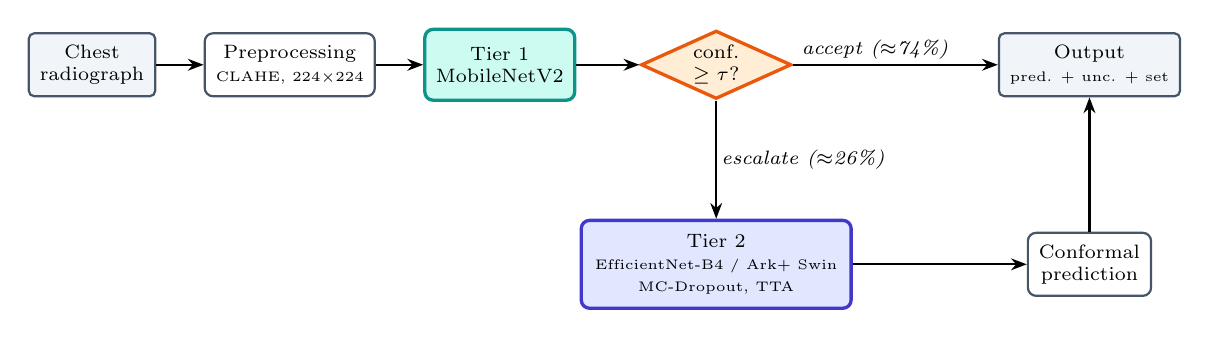
\begin{tikzpicture}
  \node[io] (input) at (0,0) {Chest\\radiograph};
  \node[proc, right=0.6cm of input] (pre) {Preprocessing\\{\tiny CLAHE, $224{\times}224$}};
  \node[light, right=0.6cm of pre] (t1) {Tier 1\\MobileNetV2};
  \node[decision, right=0.8cm of t1] (dec) {conf.\\$\geq \tau$?};
  \node[io, right=2.6cm of dec] (out) {Output\\{\tiny pred. $+$ unc. $+$ set}};
  \node[heavyblk, below=1.5cm of dec] (t2) {Tier 2\\{\tiny EfficientNet-B4 / Ark+ Swin}\\{\tiny MC-Dropout, TTA}};
  \node[proc] (cp) at (out |- t2) {Conformal\\prediction};

  \draw[flow] (input) -- (pre);
  \draw[flow] (pre) -- (t1);
  \draw[flow] (t1) -- (dec);
  \draw[flow] (dec) -- node[flowlab, above, pos=0.4]{accept ($\approx$74\%)} (out);
  \draw[flow] (dec) -- node[flowlab, right]{escalate ($\approx$26\%)} (t2);
  \draw[flow] (t2) -- (cp);
  \draw[flow] (cp) -- (out);
\end{tikzpicture}%
}
\caption{Overview of the tiered classification and confidence-based routing system. A lightweight Tier-1 screening model resolves confident cases directly; only low-confidence images are escalated to the heavier Tier-2 backbone, run with Monte~Carlo Dropout and test-time augmentation and wrapped in a conformal predictor.}\label{fig:architecture}
\end{figure}

\section{Experimental design}\label{sec:experimental}

\textbf{Datasets.} The National Institutes of Health (NIH) ChestX-Ray14 dataset \cite{wang2017chestxray} (\url{https://nihcc.app.box.com/v/ChestXray-NIHCC}) was used for the binary pneumothorax-versus-no-finding task. Table~\ref{tab:dataset} is cited before its presentation and reports patient-level splits; prevalence denotes the percentage of images labelled pneumothorax in each split. A dedicated calibration split is held out for the conformal predictor and temperature scaler, so neither is tuned on the test set. The marked class imbalance ($\approx$16.7\% prevalence) makes the area under the receiver operating characteristic curve (AUC) and sensitivity more informative than raw accuracy. The CheXpert chest-radiograph dataset \cite{irvin2019chexpert} (\url{https://stanfordmlgroup.github.io/competitions/chexpert/}) was used for zero-shot cross-dataset evaluation on its complete frontal validation cohort (202 images, $\approx$3.5\% prevalence).

\begin{table}[t]
\caption{NIH ChestX-Ray14 dataset splits.}\label{tab:dataset}
\begin{tabular}{@{}lrrrr@{}}
\toprule
Split & Images & Pneumothorax & Normal & Prevalence\\
\midrule
Train & 22,268 & 3,711 & 18,557 & 16.7\%\\
Validation & 4,772 & 796 & 3,976 & 16.7\%\\
Calibration & 1,432 & 235 & 1,197 & 16.4\%\\
Test & 4,772 & 795 & 3,977 & 16.7\%\\
\midrule
Total & 33,244 & 5,537 & 27,707 & 16.7\%\\
\botrule
\end{tabular}
\end{table}

\textbf{Preprocessing and training.} Radiographs were contrast-enhanced with contrast-limited adaptive histogram equalisation (CLAHE) \cite{zuiderveld1994contrast}, which improves local contrast while clipping amplification to limit noise, then resized to $224\times224$. Channel-wise normalisation used the ImageNet training-set means and standard deviations expected by the pretrained backbones; this places intensities on the pretraining scale and does not add ImageNet images to the medical data. Optimisation used Adam with decoupled weight decay (AdamW) \cite{loshchilov2019decoupled}; it was chosen to regularise pretrained weights independently of the adaptive gradient update. The classifier head used a tenfold higher learning rate than the pretrained backbone to learn task-specific weights while limiting destructive changes to transferred features. Early stopping used validation loss, and all runs used a fixed seed. Table~\ref{tab:hyper}, cited before its presentation, lists the pre-specified training and inference settings.

\begin{table}[t]
\caption{Training and inference hyperparameters.}\label{tab:hyper}
\begin{tabular}{@{}ll@{}}
\toprule
Hyperparameter & Value\\
\midrule
Tier-1 / Tier-2 backbone & MobileNetV2 / EfficientNet-B4 or Ark+ Swin\\
Input resolution & $224\times224$\\
Optimizer & AdamW (weight decay $10^{-4}$)\\
Backbone / head learning rate & $10^{-4}$ / $10^{-3}$\\
Batch size & 32\\
Max epochs & 50 (early stopping, patience 7)\\
MC-Dropout passes $T$ / TTA passes & 20 / 10\\
Escalation threshold $\tau$ & 0.75 (dynamic; window 50, $\delta=0.05$)\\
Conformal target coverage & $1-\alpha=0.95$\\
Random seed & 42\\
\botrule
\end{tabular}
\end{table}

\textbf{Metrics and ablations.} Discrimination is reported primarily by AUC; at the operating threshold we report accuracy, sensitivity, specificity, the $F_1$ score (the harmonic mean of precision and sensitivity) and the Matthews correlation coefficient. Calibration is summarised by the expected calibration error (ECE) over fifteen bins. For the conformal component we report empirical coverage and average prediction-set size. Fifteen configurations (A1--A15) isolate each component: single-stage baselines (A1, A2); the tiered cascade with static and dynamic thresholds (A3, A4); incremental addition of Monte~Carlo Dropout, test-time augmentation and conformal prediction (A5--A7); removal of synthetic data and of all augmentation (A8, A9); forced escalation with no routing (A10); the Ark+ backbone standalone (A11, A12); the proposed full system (A13); its zero-shot CheXpert evaluation (A14); and a variant with mixup and CutMix regularisation (A15). Every configuration is evaluated by a single unified evaluator on the same NIH test split (except A14).

\section{Results}\label{sec:results}

\textbf{Overall classification performance.} Table~\ref{tab:ablation} reports AUC, accuracy and ECE for all fifteen configurations. The highest AUC, $0.924$, is obtained by the proposed tiered system with an Ark+ Swin backbone and mixup/CutMix regularisation (A15), closely followed by the same system without that regularisation (A13, $0.923$). The lightweight Tier-1-only baseline (A1) is already highly competitive at an AUC of $0.919$ and an accuracy of $0.849$ on its own, confirming the central premise of the tiered design: a small, fast model suffices for the majority of cases, and the heavy backbone is needed only to recover the difficult remainder.

\begin{table}[t]
\caption{Ablation study on the NIH ChestX-Ray14 test set. Tier~1 is MobileNetV2 throughout; A15 attains the best AUC. ECE is reported where calibration was evaluated. A14 is a zero-shot CheXpert evaluation (lower prevalence).}\label{tab:ablation}
\begin{tabular}{@{}llrrr@{}}
\toprule
ID & Configuration & AUC & Acc. & ECE\\
\midrule
A1 & Tier 1 only (MobileNetV2) & 0.919 & 0.849 & 0.074\\
A2 & Tier 2 only (EfficientNet-B4) & 0.910 & 0.852 & 0.086\\
A3 & Tiered (static threshold) & 0.914 & 0.871 & 0.089\\
A4 & Tiered (dynamic threshold) & 0.904 & 0.881 & 0.074\\
A5 & Tiered $+$ MC Dropout & 0.909 & 0.889 & 0.055\\
A6 & Tiered $+$ MC $+$ TTA & 0.911 & 0.888 & 0.050\\
A7 & Tiered $+$ Conformal & 0.911 & 0.887 & 0.050\\
A8 & Without synthetic augmentation & 0.910 & 0.887 & 0.081\\
A9 & Without any augmentation & 0.901 & 0.887 & 0.093\\
A10 & Always Tier 2 (no routing) & 0.913 & 0.827 & 0.052\\
A11 & Tier 2 $=$ Ark+ (no MC/TTA) & 0.910 & 0.883 & 0.018\\
A12 & Tier 2 $=$ Ark+ $+$ MC $+$ TTA & 0.915 & 0.732 & 0.101\\
A13 & Proposed tiered $+$ Ark+ & \textbf{0.923} & 0.828 & --\\
A14 & Zero-shot CheXpert & 0.796 & 0.342 & --\\
A15 & Mixup/CutMix regularised & \textbf{0.924} & \textbf{0.882} & 0.060\\
\botrule
\end{tabular}
\end{table}

\textbf{Tier-2 backbone comparison.} Table~\ref{tab:backbone} compares the two candidate Tier-2 backbones with paired bootstrap 95\% confidence intervals and per-metric significance tests. The Ark+ Swin backbone achieves a higher AUC ($\Delta=+0.006$) and sensitivity ($\Delta=+0.063$, $p=0.001$), whereas EfficientNet-B4 attains higher specificity and accuracy ($\Delta=-0.027$, $p<0.001$). DeLong's paired test assesses whether two correlated receiver-operating-characteristic curves evaluated on the same cases have different areas. Here the AUC difference is not statistically significant ($p=0.203$), so the evidence is insufficient to reject equal ranking performance; the models nevertheless differ at the chosen operating point, where Ark+ is more sensitive.

\begin{table}[t]
\caption{Tier-2 backbone comparison with paired bootstrap 95\% confidence intervals. $\Delta$ is Ark+ Swin minus EfficientNet-B4.}\label{tab:backbone}
\begin{tabular}{@{}lccll@{}}
\toprule
Metric & EfficientNet-B4 & Ark+ Swin & $\Delta$ & $p$ (test)\\
\midrule
AUC & 0.910 & \textbf{0.916} & $+0.006$ & 0.203 (DeLong)\\
Accuracy & 0.852 & 0.826 & $-0.027$ & $<$0.001 (McNemar)\\
Sensitivity & 0.818 & \textbf{0.881} & $+0.063$ & 0.001 (Bootstrap)\\
Specificity & 0.859 & 0.815 & $-0.045$ & 0.001 (Bootstrap)\\
$F_1$ & 0.649 & 0.628 & $-0.021$ & 0.024 (Bootstrap)\\
\botrule
\end{tabular}
\end{table}

\textbf{Effect of the uncertainty stack and augmentation.} The incremental ablations A4--A7 improve calibration substantially while leaving discrimination unchanged: starting from the dynamic cascade (A4, ECE $0.074$), Monte~Carlo Dropout lowers the ECE to $0.055$ (A5), test-time augmentation to $0.050$ (A6), and the conformal wrapper preserves it (A7), with the AUC remaining near $0.91$ throughout. Averaging over stochastic passes and augmented views therefore makes the reported confidences trustworthy rather than making the model a better discriminator---the property required before confidences can drive a routing or abstention decision. Removing the synthetic data (A8) leaves AUC almost unchanged but raises the ECE to $0.081$, and removing all augmentation (A9) drops the AUC to $0.901$ and inflates the ECE to $0.093$; the synthetic minority-class data thus acts mainly as a calibration regulariser. Figure~\ref{fig:ablation} summarises discrimination and calibration across all configurations.

\begin{figure}[t]
\centering
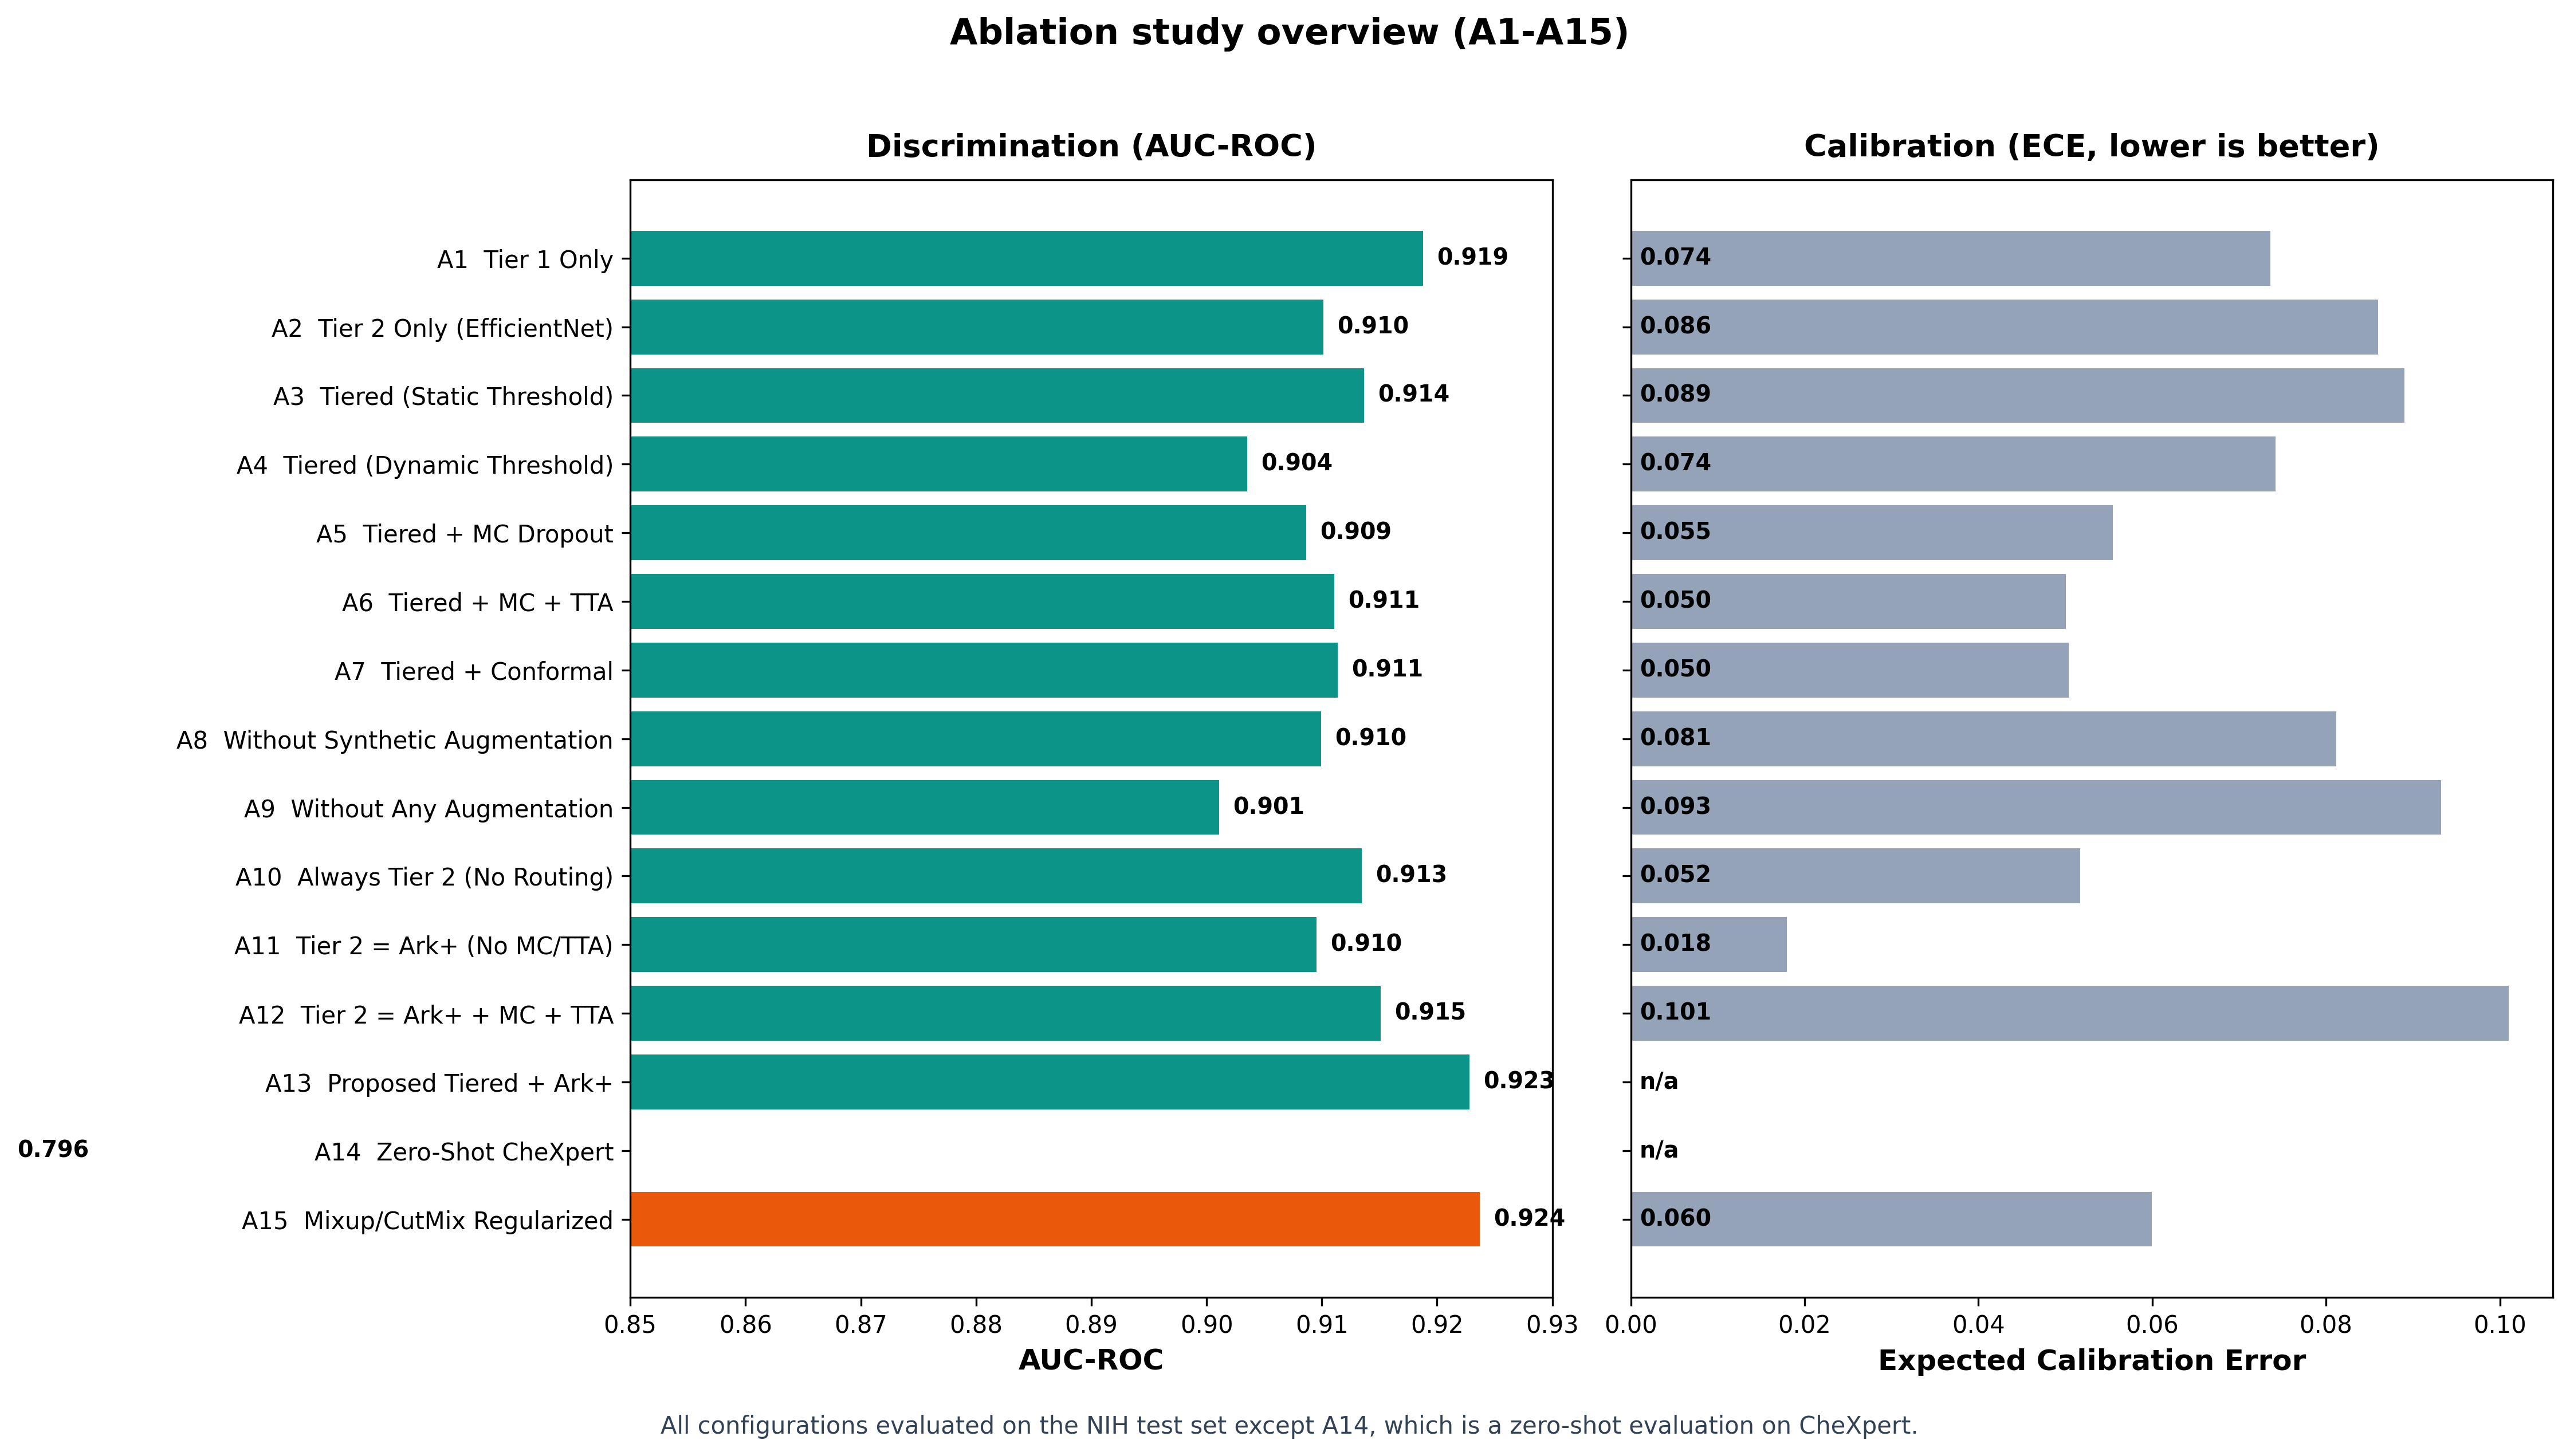
\includegraphics[width=\textwidth]{ablation_overview.png}
\caption{Discrimination (AUC, left) and calibration (ECE, right) for every configuration; the best-AUC configuration (A15) is highlighted. A14 is the zero-shot CheXpert evaluation.}\label{fig:ablation}
\end{figure}

\textbf{Routing efficiency and conformal coverage.} Forcing every image to the heavy model (A10) reaches an AUC of $0.913$ but an accuracy of only $0.827$, whereas the dynamic tiered cascade keeps accuracy above $0.88$ while escalating only about a quarter of the images, so the lightweight Tier~1 resolves roughly three quarters of cases by itself. A latency benchmark measured the MobileNetV2 tier at $5.4$\,ms per image against $17.2$\,ms for EfficientNet-B4, so the average per-image cost of the tiered system is far closer to that of the lightweight model. For the conformal component, the proposed Ark+ configuration (A15) attained an empirical coverage of $97.3\%$ at the $95\%$ target with an average prediction-set size of $1.84$ out of two classes, satisfying the guarantee while abstaining on ambiguous cases.

\textbf{Cross-dataset generalisation.} Evaluated zero-shot on the full CheXpert validation frontal cohort (A14), the threshold-free discrimination degrades only moderately (AUC $0.923\rightarrow0.796$; Fig.~\ref{fig:crossdataset}). The operating-point metrics, however, change sharply: at the fixed $0.5$ threshold the model over-predicts the positive class on CheXpert's much lower prevalence ($\approx$3.5\%), reaching a sensitivity of $1.000$ but a specificity of $0.318$. This reflects the prevalence shift interacting with an in-domain threshold and calibration, and indicates that ranking ability transfers better than a fixed operating point.

\begin{figure}[t]
\centering
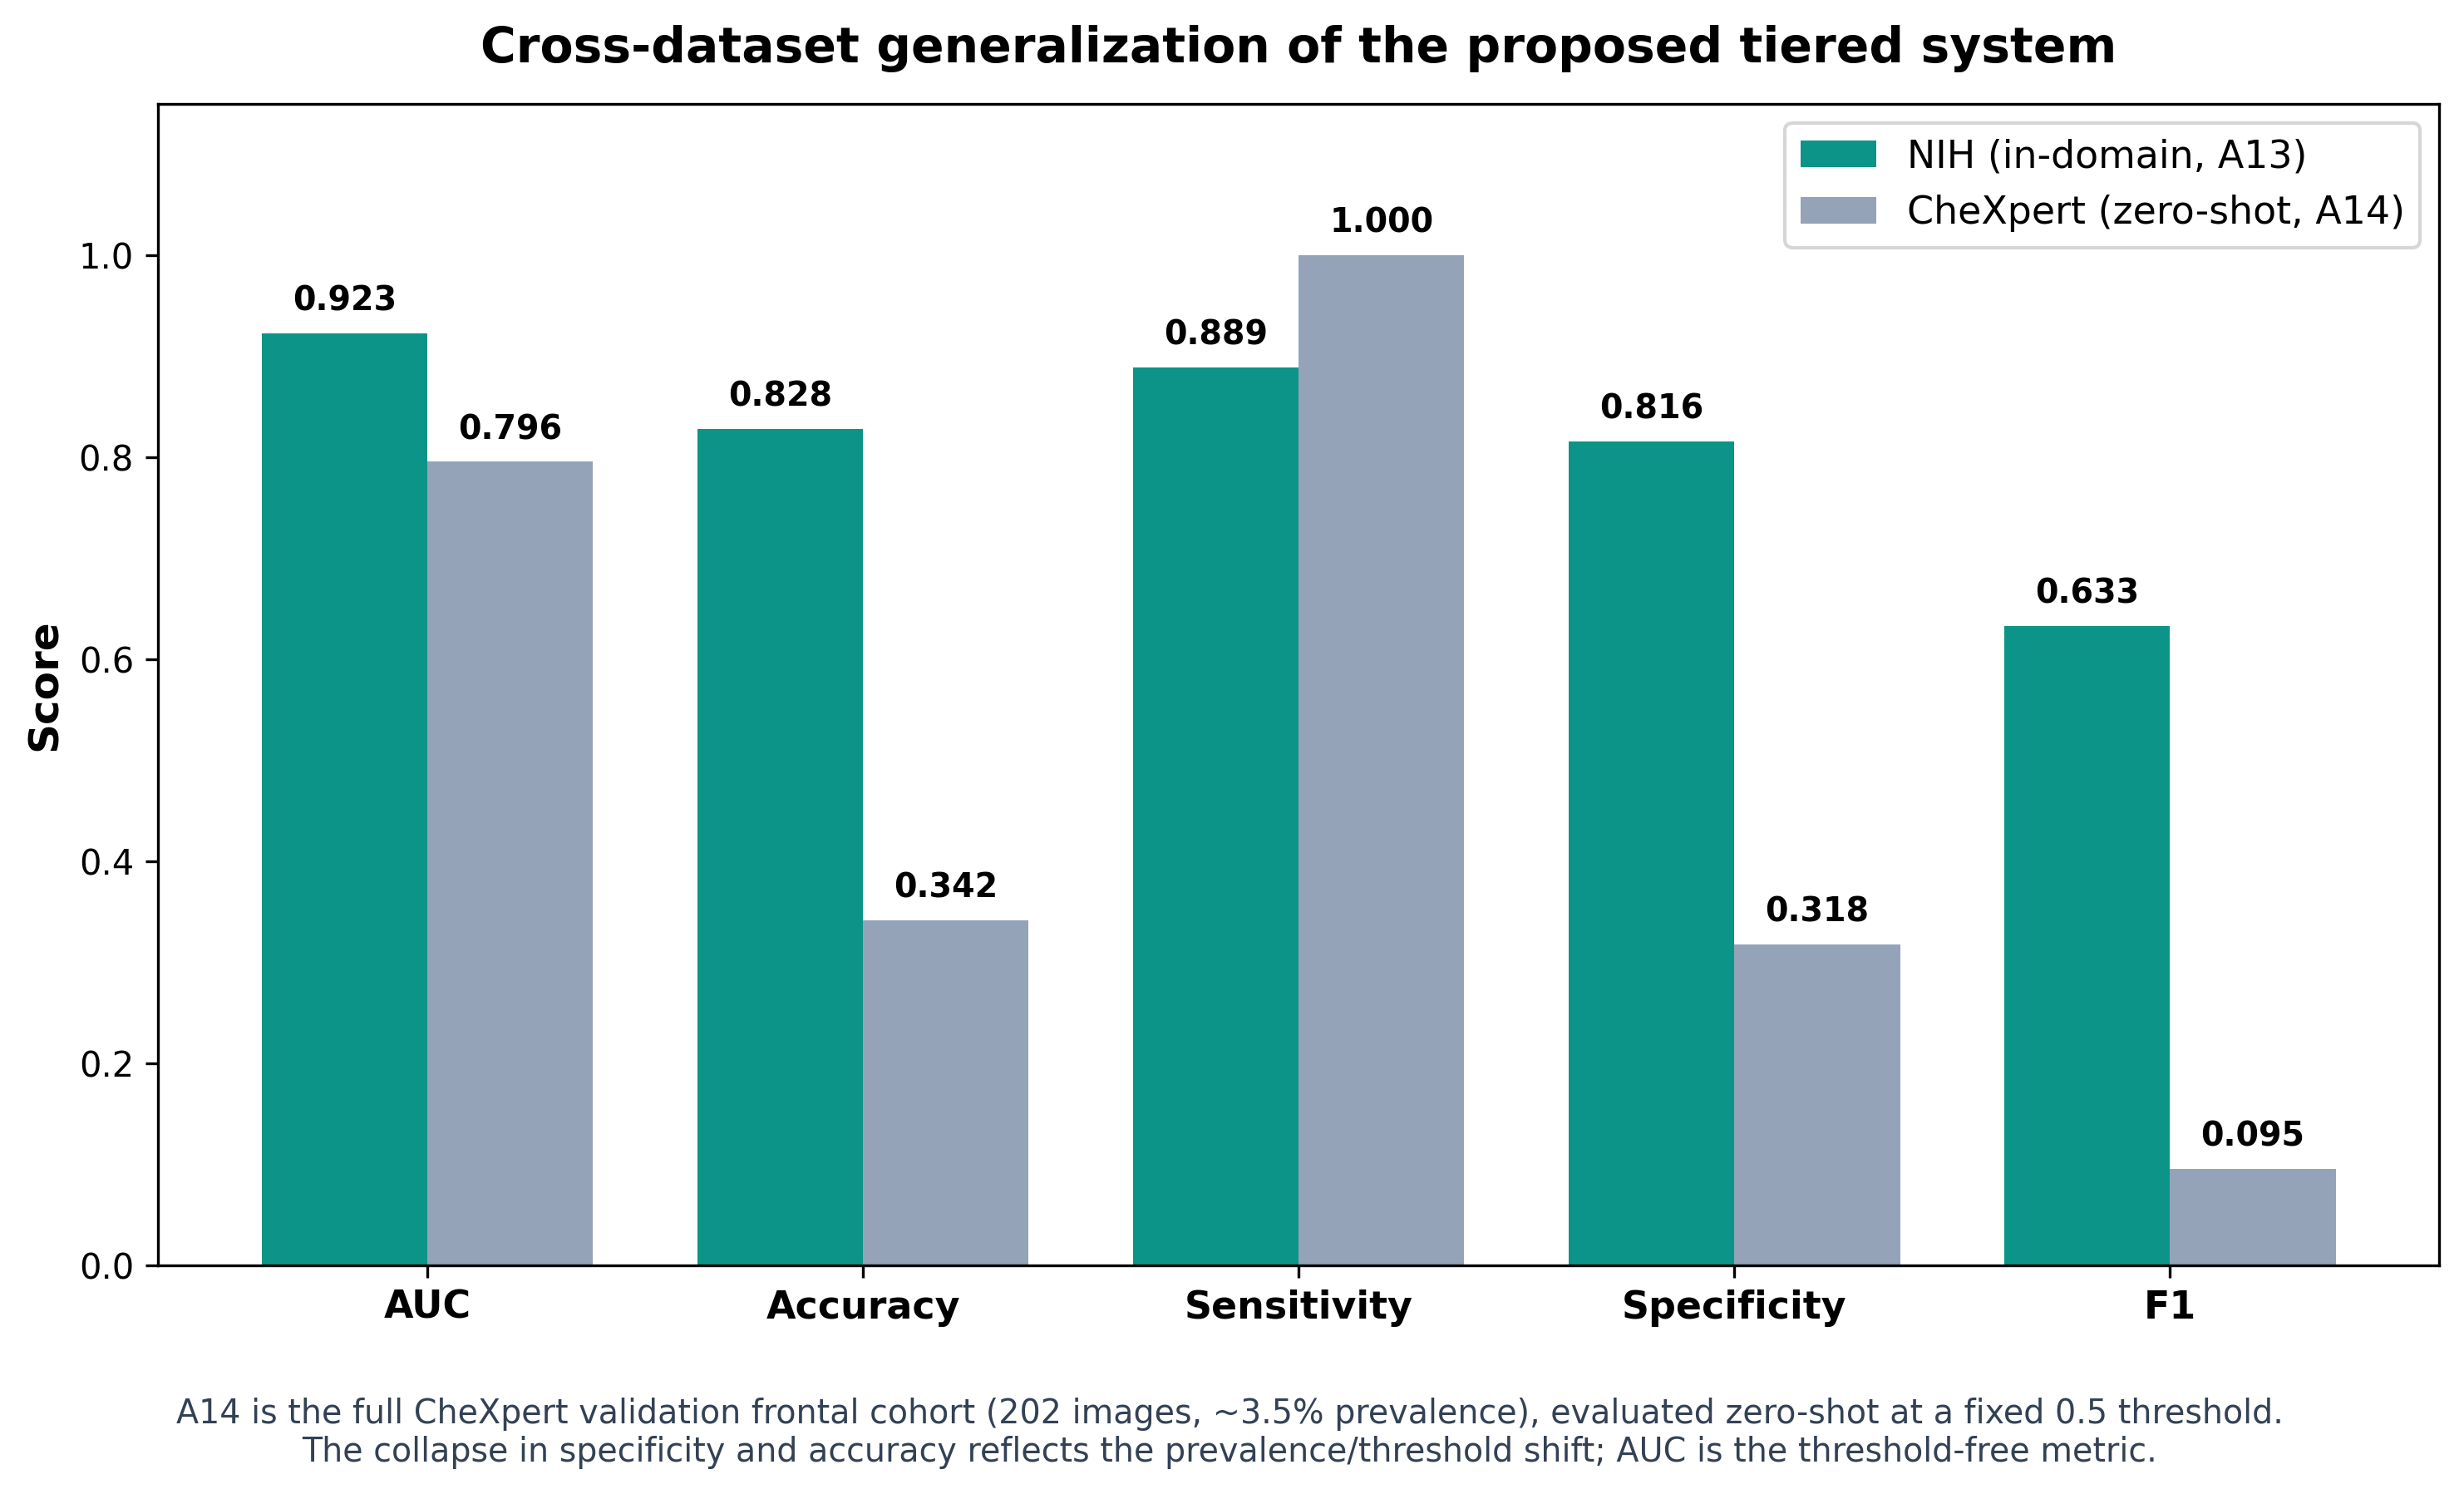
\includegraphics[width=\textwidth]{cross_dataset_generalization.png}
\caption{Cross-dataset generalisation of the proposed tiered system: in-domain NIH (A13) versus zero-shot CheXpert (A14). The area under the ROC curve degrades only moderately, whereas the operating-point metrics collapse under the prevalence shift at a fixed decision threshold.}\label{fig:crossdataset}
\end{figure}

\section{Discussion}\label{sec:discussion}

First, the tiered design retains the discrimination of the heavy model at lower average cost: Tier~1 reaches an AUC of $0.919$ and resolves approximately 74\% of cases, so the expensive backbone and uncertainty stack are invoked only for the difficult minority. This reduces average inference time and provides an explicit review path instead of forcing every image into one class.

Second, the uncertainty methods improve calibration rather than discrimination. This is the intended effect because routing and abstention depend on reliable confidence estimates. A two-label conformal set means that both classes remain plausible at the chosen coverage level and the case should be deferred; it does not mean that the system has produced two diagnoses.

Third, the foundation backbone is most useful inside the routing structure. Run standalone with the uncertainty stack on every image (A12), Ark+ is over-sensitive ($0.927$) at the expense of accuracy ($0.732$) and calibration. Inside TCR-P, Tier~1 first filters easy negatives; A13 is consequently better behaved, and the mixup/CutMix variant (A15) gives the highest AUC in the study. The dynamic threshold also exposes a trade-off: it stabilises escalation but favours specificity and depresses sensitivity in the EfficientNet cascade (A4, $0.585$), which the more sensitive Ark+ backbone recovers in the full system.

\textbf{Limitations.} The experiments identify several limitations. Audit of the current evaluation artifacts found that the reported numerical results were produced from image-level splits with patient overlap, despite the intended patient-level protocol. Consequently, all current performance estimates are provisional and must be replaced after retraining on mutually exclusive patient-level train, validation, calibration and test splits. Independently, the cross-dataset evaluation suggests limited transfer of both ranking performance and the in-domain operating threshold: at a fixed threshold the model over-predicts the positive class under CheXpert's lower prevalence. The reported sensitivity of $1.000$ reflects only seven positive cases in the 202-image validation cohort and should not be interpreted as perfect clinical sensitivity. The conformal prediction sets are conservative, with an average set size of $1.84$--$2.00$, and the routing threshold remains a heuristic hyperparameter. The task is restricted to binary pneumothorax detection on frontal radiographs, while report-mined NIH labels introduce additional noise.

Future work follows these limitations. The heuristic escalation threshold should be replaced by a learned policy optimising a clinical objective; adaptive conformal sets may reduce average set size while preserving coverage; the binary task should be extended to multi-label, multi-pathology prediction; and further external sites should be evaluated with site-specific recalibration.

\section{Conclusion}\label{sec:conclusion}

We proposed Tiered Confidence Routing for Pneumothorax (TCR-P), which pairs a lightweight MobileNetV2 screening stage with a heavier EfficientNet-B4 or Ark+ Swin stage and adds Monte~Carlo Dropout, test-time augmentation, temperature scaling and conformal prediction. A fifteen-configuration ablation study showed that Tier~1 resolves approximately 74\% of cases, the uncertainty stack reduces expected calibration error from $0.074$ to $0.050$ while AUC remains near $0.91$, and the best TCR-P configuration reaches an AUC of $0.924$ with 97.3\% empirical coverage at the 95\% conformal target.

The results support TCR-P as a selective-computation research prototype, not a clinically validated diagnostic device; prospective multi-site validation is required before deployment.

\section*{Acknowledgements}

The authors thank their institutional colleagues and academic supervisors for their feedback on the study and manuscript.

\section*{Code and data availability}

All code, trained-model configurations and evaluation scripts are available on GitHub at \url{https://github.com/xdboi123yes/xray} (placeholder repository, to be migrated to the corresponding author's account). The study uses the publicly available NIH ChestX-Ray14 \cite{wang2017chestxray} and CheXpert \cite{irvin2019chexpert} datasets.

%% --- Bibliography embedded directly (Nature Portfolio submission format).
%% No BibTeX run is needed; references.bib is kept for the record / regeneration.
%% To regenerate, restore the bibliography command (references.bib) and run bibtex.
\begin{thebibliography}{10}
\expandafter\ifx\csname url\endcsname\relax
  \def\url#1{\burl{#1}}\fi
\expandafter\ifx\csname urlprefix\endcsname\relax\def\urlprefix{URL }\fi
\providecommand{\bibinfo}[2]{#2}
\providecommand{\eprint}[2][]{\url{#2}}
\providecommand{\doi}[1]{\url{https://doi.org/#1}}
\bibcommenthead

\bibitem{rajpurkar2017chexnet}
\bibinfo{author}{Rajpurkar, P.} \emph{et~al.}
\newblock \bibinfo{title}{Chexnet: Radiologist-level pneumonia detection on
  chest x-rays with deep learning}.
\newblock \emph{\bibinfo{journal}{arXiv preprint arXiv:1711.05225}}
  (\bibinfo{year}{2017}).

\bibitem{irvin2019chexpert}
\bibinfo{author}{Irvin, J.} \emph{et~al.}
\newblock \emph{\bibinfo{title}{Chexpert: A large chest radiograph dataset with
  uncertainty labels and expert comparison}}, Vol.~\bibinfo{volume}{33},
  \bibinfo{pages}{590--597} (\bibinfo{year}{2019}).

\bibitem{sandler2018mobilenetv2}
\bibinfo{author}{Sandler, M.}, \bibinfo{author}{Howard, A.},
  \bibinfo{author}{Zhu, M.}, \bibinfo{author}{Zhmoginov, A.} \&
  \bibinfo{author}{Chen, L.-C.}
\newblock \emph{\bibinfo{title}{Mobilenetv2: Inverted residuals and linear
  bottlenecks}}, \bibinfo{pages}{4510--4520} (\bibinfo{year}{2018}).

\bibitem{tan2019efficientnet}
\bibinfo{author}{Tan, M.} \& \bibinfo{author}{Le, Q.}
\newblock \emph{\bibinfo{title}{Efficientnet: Rethinking model scaling for
  convolutional neural networks}}, \bibinfo{pages}{6105--6114}
  (\bibinfo{organization}{PMLR}, \bibinfo{year}{2019}).

\bibitem{ma2025arkplus}
\bibinfo{author}{Ma, D.}, \bibinfo{author}{Pang, J.}, \bibinfo{author}{Gotway,
  M.~B.} \& \bibinfo{author}{Liang, J.}
\newblock \bibinfo{title}{A fully open ai foundation model applied to chest
  radiography}.
\newblock \emph{\bibinfo{journal}{Nature}} \textbf{\bibinfo{volume}{643}},
  \bibinfo{pages}{488--498} (\bibinfo{year}{2025}).

\bibitem{liu2021swin}
\bibinfo{author}{Liu, Z.} \emph{et~al.}
\newblock \emph{\bibinfo{title}{Swin transformer: Hierarchical vision
  transformer using shifted windows}}, \bibinfo{pages}{10012--10022}
  (\bibinfo{year}{2021}).

\bibitem{gal2016dropout}
\bibinfo{author}{Gal, Y.} \& \bibinfo{author}{Ghahramani, Z.}
\newblock \emph{\bibinfo{title}{Dropout as a bayesian approximation:
  Representing model uncertainty in deep learning}},
  \bibinfo{pages}{1050--1059} (\bibinfo{organization}{PMLR},
  \bibinfo{year}{2016}).

\bibitem{vovk2005algorithmic}
\bibinfo{author}{Vovk, V.}, \bibinfo{author}{Gammerman, A.} \&
  \bibinfo{author}{Shafer, G.}
\newblock \emph{\bibinfo{title}{Algorithmic learning in a random world}}
  (\bibinfo{publisher}{Springer Science \& Business Media},
  \bibinfo{year}{2005}).

\bibitem{shafer2008tutorial}
\bibinfo{author}{Shafer, G.} \& \bibinfo{author}{Vovk, V.}
\newblock \bibinfo{title}{A tutorial on conformal prediction}.
\newblock \emph{\bibinfo{journal}{Journal of Machine Learning Research}}
  \textbf{\bibinfo{volume}{9}} (\bibinfo{year}{2008}).

\bibitem{rombach2022high}
\bibinfo{author}{Rombach, R.}, \bibinfo{author}{Blattmann, A.},
  \bibinfo{author}{Lorenz, D.}, \bibinfo{author}{Esser, P.} \&
  \bibinfo{author}{Ommer, B.}
\newblock \emph{\bibinfo{title}{High-resolution image synthesis with latent
  diffusion models}}, \bibinfo{pages}{10684--10695} (\bibinfo{year}{2022}).

\bibitem{wang2017chestxray}
\bibinfo{author}{Wang, X.} \emph{et~al.}
\newblock \emph{\bibinfo{title}{Chestx-ray8: Hospital-scale chest x-ray
  database and benchmarks on weakly-supervised classification and localization
  of common thorax diseases}}, \bibinfo{pages}{2097--2106}
  (\bibinfo{year}{2017}).

\bibitem{litjens2017survey}
\bibinfo{author}{Litjens, G.} \emph{et~al.}
\newblock \bibinfo{title}{A survey on deep learning in medical image analysis}.
\newblock \emph{\bibinfo{journal}{Medical image analysis}}
  \textbf{\bibinfo{volume}{42}}, \bibinfo{pages}{60--88}
  (\bibinfo{year}{2017}).

\bibitem{wang2019aleatoric}
\bibinfo{author}{Wang, G.} \emph{et~al.}
\newblock \bibinfo{title}{Aleatoric uncertainty estimation with test-time
  augmentation for medical image segmentation with convolutional neural
  networks}.
\newblock \emph{\bibinfo{journal}{Neurocomputing}}
  \textbf{\bibinfo{volume}{338}}, \bibinfo{pages}{34--45}
  (\bibinfo{year}{2019}).

\bibitem{guo2017calibration}
\bibinfo{author}{Guo, C.}, \bibinfo{author}{Pleiss, G.}, \bibinfo{author}{Sun,
  Y.} \& \bibinfo{author}{Weinberger, K.~Q.}
\newblock \emph{\bibinfo{title}{On calibration of modern neural networks}},
  \bibinfo{pages}{1321--1330} (\bibinfo{organization}{PMLR},
  \bibinfo{year}{2017}).

\bibitem{romano2020classification}
\bibinfo{author}{Romano, Y.}, \bibinfo{author}{Sesia, M.} \&
  \bibinfo{author}{Cand{\`e}s, E.}
\newblock \emph{\bibinfo{title}{Classification with valid and adaptive
  coverage}}, Vol.~\bibinfo{volume}{33}, \bibinfo{pages}{3581--3591}
  (\bibinfo{year}{2020}).

\bibitem{angelopoulos2021uncertainty}
\bibinfo{author}{Angelopoulos, A.~N.}, \bibinfo{author}{Bates, S.},
  \bibinfo{author}{Jordan, M.} \& \bibinfo{author}{Malik, J.}
\newblock \emph{\bibinfo{title}{Uncertainty sets for image classifiers using
  conformal prediction}} (\bibinfo{year}{2021}).

\bibitem{angelopoulos2023gentle}
\bibinfo{author}{Angelopoulos, A.~N.} \& \bibinfo{author}{Bates, S.}
\newblock \bibinfo{title}{A gentle introduction to conformal prediction and
  distribution-free uncertainty quantification}.
\newblock \emph{\bibinfo{journal}{Foundations and Trends in Machine Learning}}
  \textbf{\bibinfo{volume}{16}}, \bibinfo{pages}{494--591}
  (\bibinfo{year}{2023}).

\bibitem{zhang2018mixup}
\bibinfo{author}{Zhang, H.}, \bibinfo{author}{Cisse, M.},
  \bibinfo{author}{Dauphin, Y.~N.} \& \bibinfo{author}{Lopez-Paz, D.}
\newblock \emph{\bibinfo{title}{mixup: Beyond empirical risk minimization}}
  (\bibinfo{year}{2018}).

\bibitem{yun2019cutmix}
\bibinfo{author}{Yun, S.} \emph{et~al.}
\newblock \emph{\bibinfo{title}{Cutmix: Regularization strategy to train strong
  classifiers with localizable features}}, \bibinfo{pages}{6023--6032}
  (\bibinfo{year}{2019}).

\bibitem{selvaraju2017gradcam}
\bibinfo{author}{Selvaraju, R.~R.} \emph{et~al.}
\newblock \emph{\bibinfo{title}{Grad-cam: Visual explanations from deep
  networks via gradient-based localization}}, \bibinfo{pages}{618--626}
  (\bibinfo{year}{2017}).

\bibitem{draelos2020hirescam}
\bibinfo{author}{Draelos, R.~L.} \& \bibinfo{author}{Carin, L.}
\newblock \bibinfo{title}{Use hirescam instead of grad-cam for faithful
  explanations of convolutional neural networks}.
\newblock \emph{\bibinfo{journal}{arXiv preprint arXiv:2011.08891}}
  (\bibinfo{year}{2020}).

\bibitem{zuiderveld1994contrast}
\bibinfo{author}{Zuiderveld, K.}
\newblock \bibinfo{title}{ in \textit{Contrast limited adaptive histogram
  equalization}}  \bibinfo{pages}{474--485} (\bibinfo{publisher}{Academic Press
  Professional}, \bibinfo{year}{1994}).

\bibitem{loshchilov2019decoupled}
\bibinfo{author}{Loshchilov, I.} \& \bibinfo{author}{Hutter, F.}
\newblock \emph{\bibinfo{title}{Decoupled weight decay regularization}}
  (\bibinfo{year}{2019}).

\end{thebibliography}

\end{document}
